% Options for packages loaded elsewhere
\PassOptionsToPackage{unicode}{hyperref}
\PassOptionsToPackage{hyphens}{url}
%
\documentclass[
]{article}
\usepackage{amsmath,amssymb}
\usepackage{lmodern}
\usepackage{iftex}
\usepackage{graphicx}
\usepackage{float}
\usepackage{ngerman}
\usepackage[a4paper, total={6in, 8in}]{geometry}
\ifPDFTeX
  \usepackage[T1]{fontenc}
  \usepackage[utf8]{inputenc}
  \usepackage{textcomp} % provide euro and other symbols
\else % if luatex or xetex
  \usepackage{unicode-math}
  \defaultfontfeatures{Scale=MatchLowercase}
  \defaultfontfeatures[\rmfamily]{Ligatures=TeX,Scale=1}
\fi
% Use upquote if available, for straight quotes in verbatim environments
\IfFileExists{upquote.sty}{\usepackage{upquote}}{}
\IfFileExists{microtype.sty}{% use microtype if available
  \usepackage[]{microtype}
  \UseMicrotypeSet[protrusion]{basicmath} % disable protrusion for tt fonts
}{}
\makeatletter
\@ifundefined{KOMAClassName}{% if non-KOMA class
  \IfFileExists{parskip.sty}{%
    \usepackage{parskip}
  }{% else
    \setlength{\parindent}{0pt}
    \setlength{\parskip}{6pt plus 2pt minus 1pt}}
}{% if KOMA class
  \KOMAoptions{parskip=half}}
\makeatother
\usepackage{xcolor}
\IfFileExists{xurl.sty}{\usepackage{xurl}}{} % add URL line breaks if available
\IfFileExists{bookmark.sty}{\usepackage{bookmark}}{\usepackage{hyperref}}
\hypersetup{
  pdftitle={arc42 Template},
  hidelinks,
  pdfcreator={LaTeX via pandoc}}
\urlstyle{same} % disable monospaced font for URLs
\usepackage{longtable,booktabs,array}
\usepackage{calc} % for calculating minipage widths
% Correct order of tables after \paragraph or \subparagraph
\usepackage{etoolbox}
\makeatletter
\patchcmd\longtable{\par}{\if@noskipsec\mbox{}\fi\par}{}{}
\makeatother
% Allow footnotes in longtable head/foot
\IfFileExists{footnotehyper.sty}{\usepackage{footnotehyper}}{\usepackage{footnote}}
\makesavenoteenv{longtable}
\usepackage{graphicx}
\makeatletter
\def\maxwidth{\ifdim\Gin@nat@width>\linewidth\linewidth\else\Gin@nat@width\fi}
\def\maxheight{\ifdim\Gin@nat@height>\textheight\textheight\else\Gin@nat@height\fi}
\makeatother
% Scale images if necessary, so that they will not overflow the page
% margins by default, and it is still possible to overwrite the defaults
% using explicit options in \includegraphics[width, height, ...]{}
\setkeys{Gin}{width=\maxwidth,height=\maxheight,keepaspectratio}
% Set default figure placement to htbp
\makeatletter
\def\fps@figure{htbp}
\makeatother
\setlength{\emergencystretch}{3em} % prevent overfull lines
\providecommand{\tightlist}{%
  \setlength{\itemsep}{0pt}\setlength{\parskip}{0pt}}
\setcounter{secnumdepth}{-\maxdimen} % remove section numbering
\ifLuaTeX
  \usepackage{selnolig}  % disable illegal ligatures
\fi

\usepackage[citestyle=numeric, sorting=none]{biblatex}


\addbibresource{Literatur.bib}

\title{
  \begin{center}
    
\includegraphics[width=0.5\textwidth]{resources/header.png} \\
    Projektbericht Trashpong
  \end{center}
}
\author{Aron Seidl, Maylis Grune, Carolin Enderlein}
\date{Januar 2023}

\begin{document}
\maketitle

% DOCUMENT STARTS HERE
\hypertarget{section-introduction-and-goals}{%
\section{Architektur}\label{section-introduction-and-goals}}

Im Rahmen der Architektur wird eine zentralisierte Architektur verwendet, wobei es sich um eine Client-Server-Architektur handelt (vgl. Abbildung \ref{fig:clientserver}).
Die Programmteile werden in zwei Einheiten unterteilt, um eine klare Trennung zu gewährleisten. 
Der Server stellt einen bestimmten Service bereit und leitet die Anfragen an die Clients weiter. 
Die Clients empfangen diese Anfragen.\cite{tanenbaum2007distributed}
Der Client ist eine kompilierte Anwendung, geschrieben in der Open-Source Godot Engine \cite{godot}, welcher die
Services des Servers nutzt. 
Die Verteilung der Anwendungslogik, auf Client und Server, wird durch die (Abbildung \ref{fig:destribution-of-logic}) verdeutlicht.
Der Client besitzt dabei die gesamte Spiellogik, über die der Benutzer das Spiel spielen kann. 
Die Benutzerschnittstelle ist hierbei die kompilierte Godot Anwendung, welche die Spiellogik implementiert.

\begin{figure}[H]
	\centering
	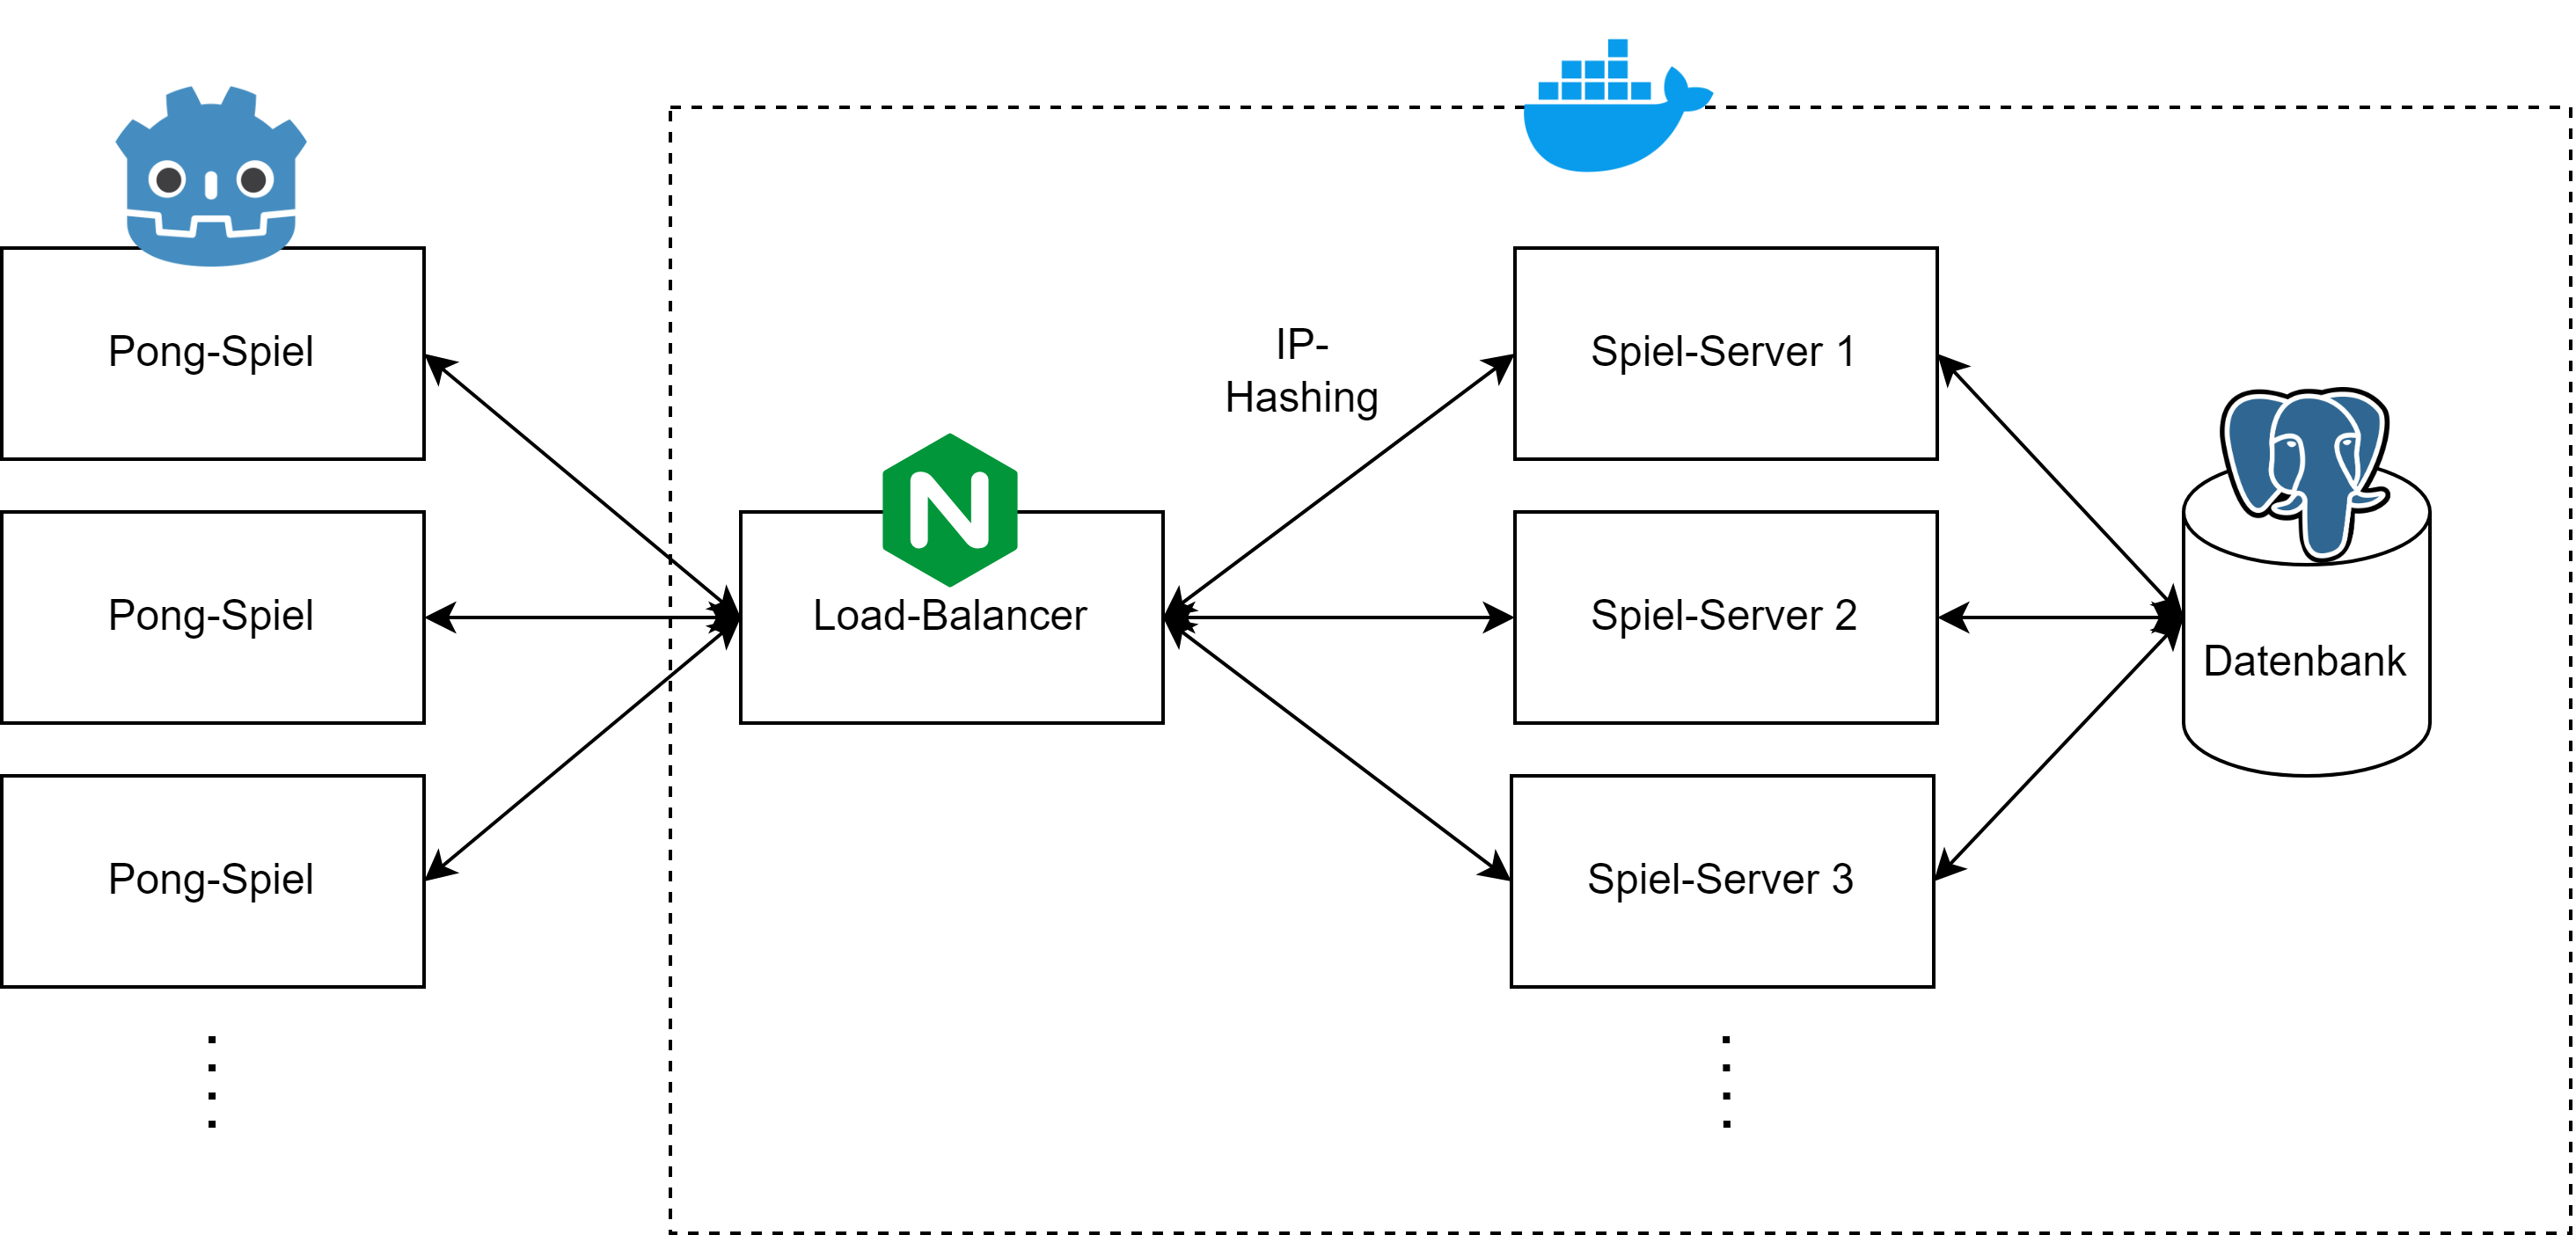
\includegraphics[width=0.8\textwidth ]{resources/Client-Server.drawio.png}
	\caption{Kontext-Sicht der Client-Server-Architektur des Pong Spiels}
	\label{fig:clientserver}
\end{figure}

Um Daten zu erhalten, sendet die Anwendung Anfragen an die REST API, welche Anwendungslogik implementiert hat um mit der Datenbank zu interagieren.
Die Benutzeranwendung muss zudem eigene Logik implementieren, da diese aufgrund von Echtzeit Anforderungen nicht auf einen Server warten kann.
Komponenten mit Echtzeit Anforderungen, die das  Rendering, die Übernahme von Benutzereingaben müssen auf dem Client Computer ausgeführt werden.
Server wie auch Client besitzen demnach ihre eigene Anwendungslogik, die sich auf die jeweiligen Anforderungen spezialisiert haben.

\begin{figure}[H]
	\centering
	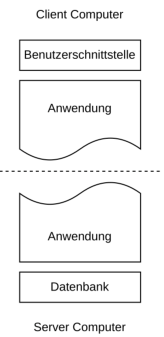
\includegraphics[width=0.6\textwidth ]{resources/server_client.pdf}
	\caption{Aufteilung der Anwendungslogik in Client und Server}
	\label{fig:destribution-of-logic}
\end{figure}

Der Server kann über eine Docker Compose bereitgestellt werden.
Innerhalb dieses Deployments wird eine Postgres-Datenbank, 
ein Nginx-Load-Balancer und ein beliebig skalierbarer Spieleserver, welcher die Anfragen der Clients verarbeitet, bereitgestellt.

\subsection{Server Architektur}
\begin{figure}[H]
	\centering
	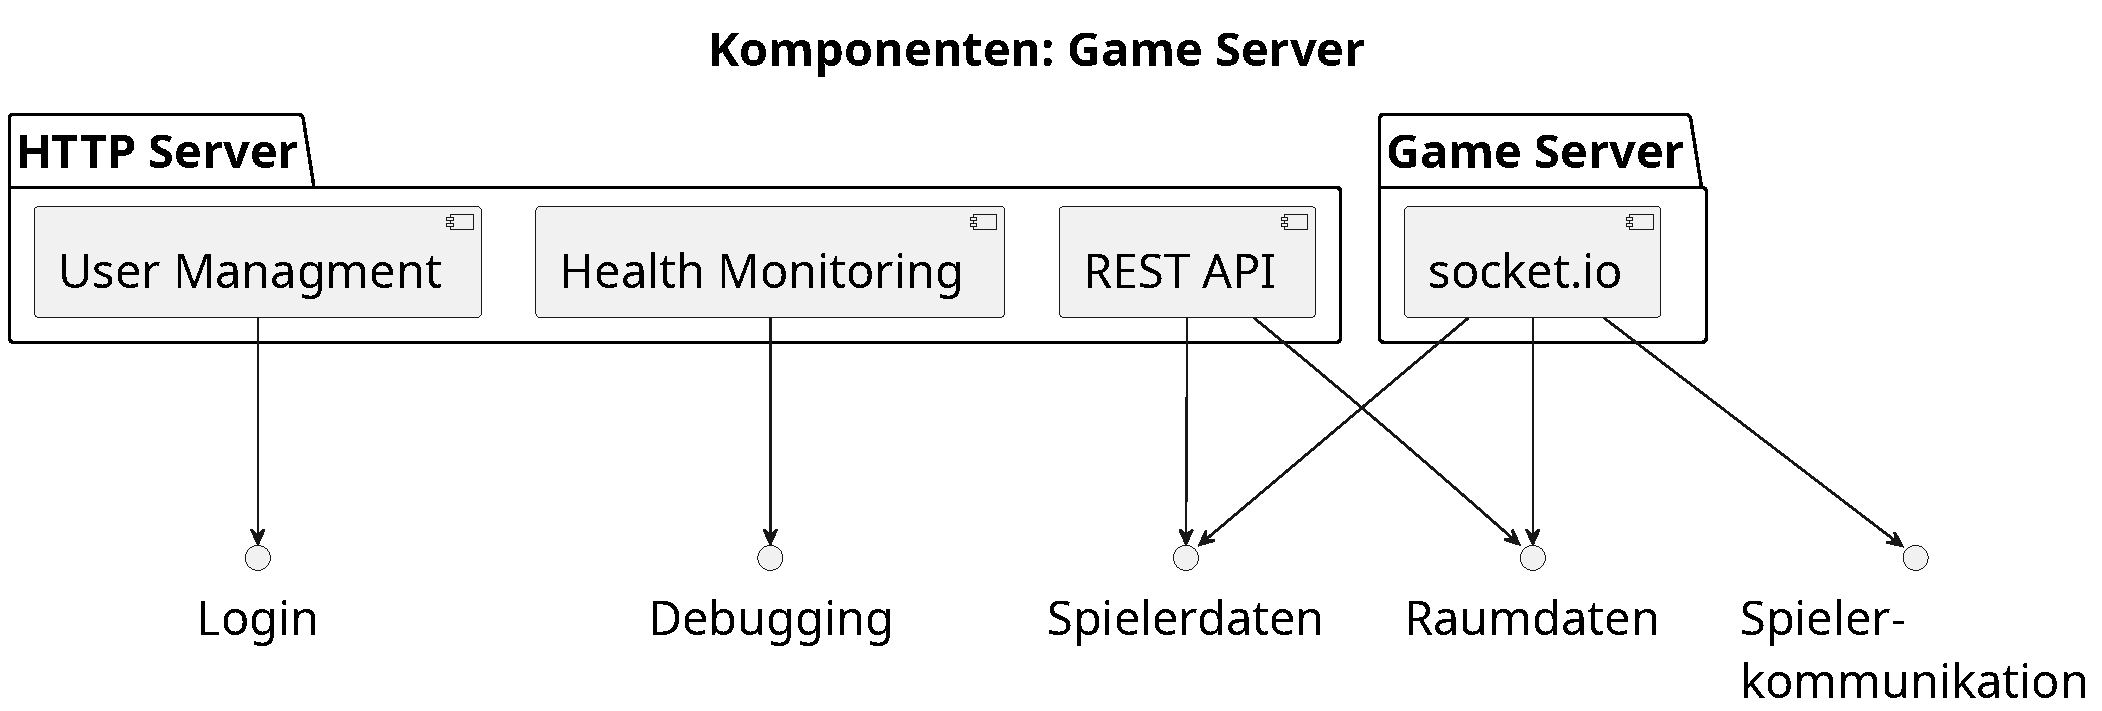
\includegraphics[width=\textwidth ]{resources/game_server.pdf}
	\caption{Komponentensicht der Serveranwendung}
	\label{fig:server}
\end{figure}

Der Server besteht aus zwei Komponenten, dem HTTP Server und dem Game Server.
Der HTTP Server verfolgt dabei eine \glqq  [..] client-server Interaktion, auch bekannt als 
request-reply Verhalten [..]\grqq{}\cite[S.37 ff.]{tanenbaum2007distributed}.
Diese Komponente, wie sie in (Abbildung \ref{fig:server}) dargestellt ist,
bietet dem Client Benutzerschnittstellen an um sich anzumelden, Räume zu erstellen und diesen beizutreten.
Der HTTP Server ist dabei verbindungslos, das bedeutet, 
dass der Server nachdem er die Anfrage bearbeitet hat, die Verbindung schließt.
Der Server hat dabei keine Referenz zu dem Client, der die Anfrage gestellt hat.
Was für Anwendung, die Daten bereitstellen sollen die einfachste Form der Kommunikation dargestellt.

Innerhalb des Spiels, sind verbindungslose Protokolle nicht ausreichend, da hier eine Echtzeitkommunikation benötigt wird.
Websockets wären hier ein Protokoll, welches einen verbindungsorientierten Ansatz verfolgt.
Diese \glqq [..] verwenden eine einzelne TCP-Verbindung für den Datenverkehr in beide Richtungen. 
\grqq{} \cite[Kapitel 1.1]{rfc-websocket}.
Somit kann mit Websockets ein bidirektionaler Kommunikationskanal aufgebaut werden mit dem die Clients 
und der Server in Echtzeit kommunizieren können.
Spieleinformationen können so zwischen den Clients ausgetascht werden. 
Der Server wird dabei als Vermittler verwendet. Um dies zu ermöglichen wird die Socket.io Bibliothek verwendet.
Socket.io ergänzt das Websocket Protokoll und ermöglicht es Räume zu erstellen und zu verwalten.
Damit können mehrere Clients innerhalb eines Raums miteinander kommunizieren.

Die Datenbank speichert die Räume, in denen die Spieler ihr Spiel spielen. 
Jeder Spieler kann Räume erstellen und ihnen beitreten und gehört somit diesen 
Räumen an (vgl. Abbildung \ref{fig:ER-Modell}).
Ein Spieler kann dabei mehrere Räume erstellen, so ist es diesem auch möglich, in mehreren Räumen gleichzeitig zu sein.
Zum Zeitpunkt des Spiels kann der Spieler nur in einem Raum sein.

Zum Ausgleichen von Anfragen wird ein Nginx Load Balancer verwendet.
Dieser verteilt die Anfragen auf die verschiedenen Serverinstanzen.
Da für die Echtzeitkommunikation Websockets verwendet werden, ist es notwendig,
dass der Verbindung eines Clients immer auf die gleiche Serverinstanz leiten.
Dafür wird für die Verteilung der Anfragen IP-Hashing verwendet.
Der Load Balancer speichert dabei die IP-Adresse des Clients und 
leitet die Anfragen immer an die gleiche Serverinstanz weiter.

\begin{figure}[H]
	\centering
	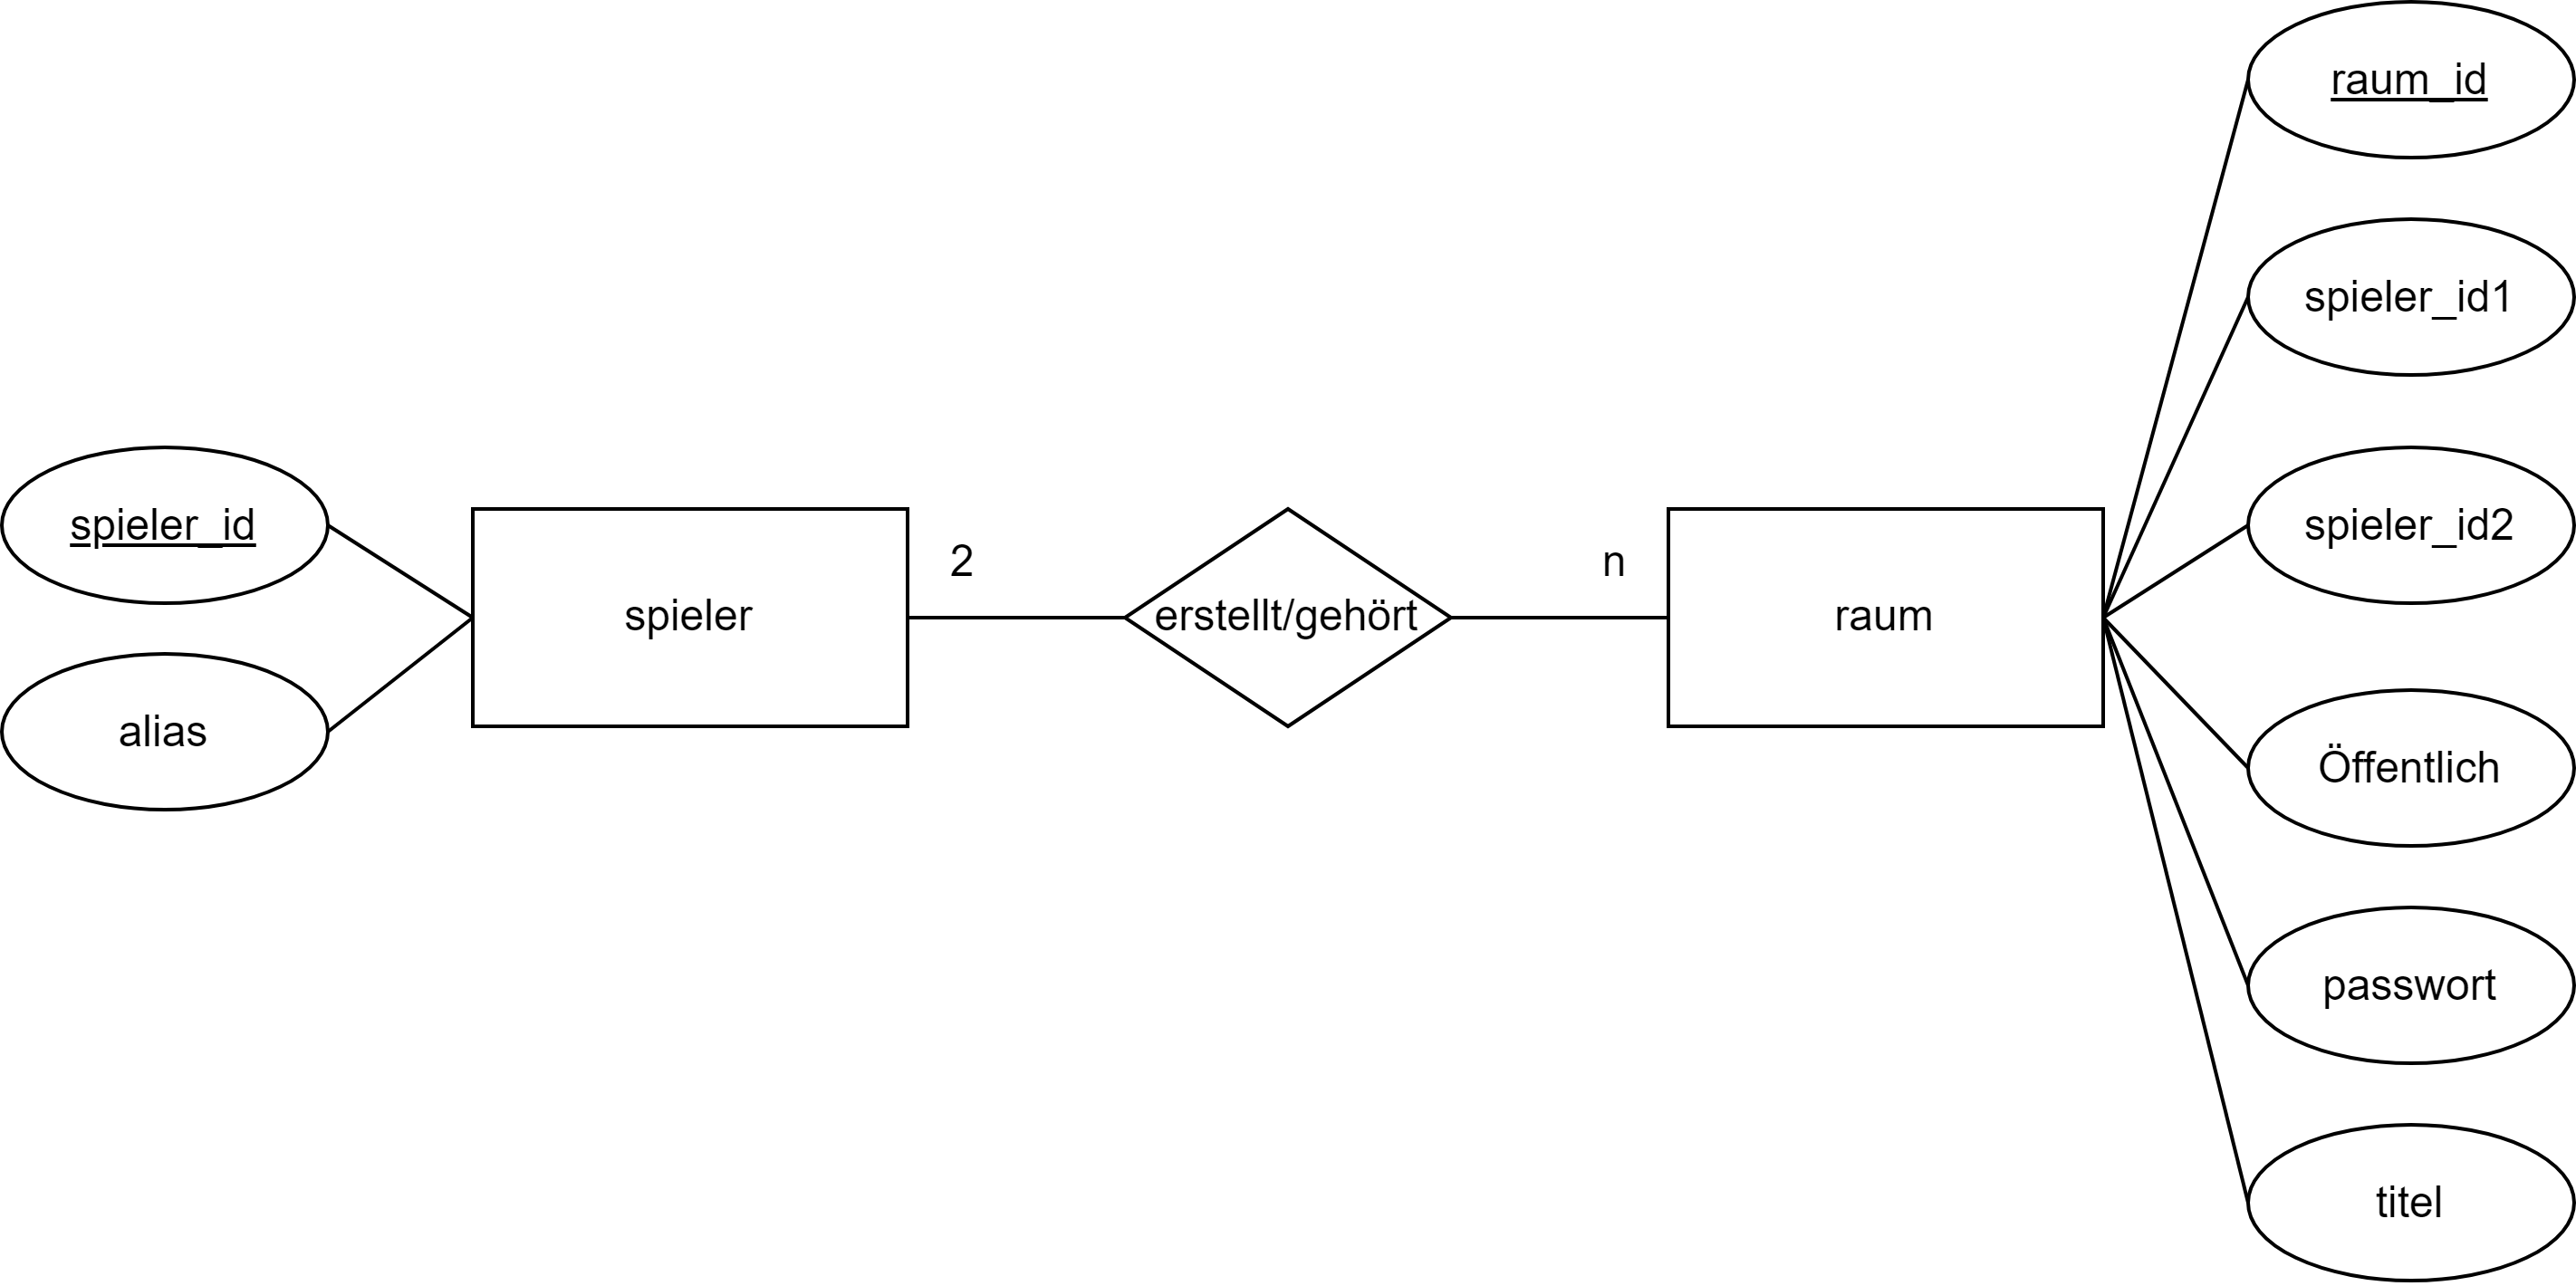
\includegraphics[width=\textwidth ]{resources/ER-Modell.png}
	\caption{ER-Modell der Datenbankarchitektur}
	\label{fig:ER-Modell}
\end{figure}

\subsection{Client Architektur}
\begin{figure}[H]
	\centering
	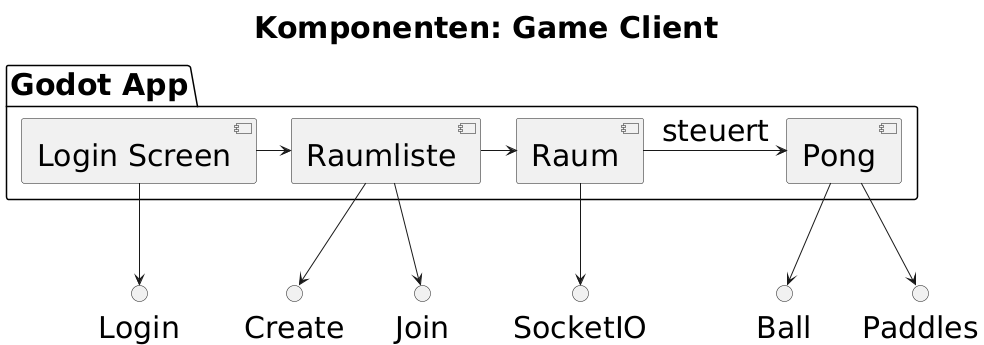
\includegraphics[width=\textwidth -80pt ]{resources/Client-Architektur.png}
	\caption{Komponentensicht des Clients.}
	\label{fig:clientarchitektur}
\end{figure}
Der Client besteht aus 4 Komponenten. Im Login Screen authentifiziert sich der Client mit dem Server verbindungslos. Auch das Erstellen und Betreten der Räume ist nur über REST-Anfragen gehandlet. Erst wenn ein Spieler den Raum beitritt wird mit Websockets ein bi-direktionaler Kommunikationskanal erstellt (vgl. Server Architektur). Über diesen Kanal werden dann die Spielelemente des Pong Spiels gesteuert. 


\hypertarget{section-achitactural-decision}{
\subsection{Architektur Entscheidung}}

\glqq Viele Client-Server-Anwendung sind grundsetzlich aus drei unterschiedlichen Komponenten zusammengesetzt[...]\grqq{} \cite[S.57 ff.]{tanenbaum2007distributed}.
Die Clients interagieren daher auch mit einer Benutzerschnittstelle. Dabei handelt es sich um ein HTTP Server, der die Anfragen der Clients entgegennimmt.
Der HTTP Server unterstützen dabei HTTP Anfragen, genauso wie Websocketverbindungen.
Diese wiederum interagiert dabei mit \glqq Controllern \grqq{}, die die Logik der Anwendung implementieren und welche dann
mit der Datenhaltung interagieren. Damit kann eine klare Trennung von Datenhaltung und Logik erreicht werden, welches die Anwendung
modular macht. Es können dadurch andere Datenbanksysteme verwendet werden, ohne dass die Logik der Anwendung angepasst werden muss.

Innerhalb der Server Applikation wird auf zwei Paradigmen.
Einerseits wird auf das request-reply Paradigma gesetzt, um Nutzer zu autorisieren, Räume zu erstellen und zu verwalten.
Hierbei ist keine Echtzeitkommunikation notwendig, da die Anfragen nur einmalig durchgeführt werden.
Auf der Game Server Seite wurde sich dabei für eine nachrichtenbasierte Kommunikation entschieden, 
um die Anforderungen der Echtzeitkommunikation zu erfüllen. Diese Entscheidung wurde getroffen, 
weil synchrone Kommunikationsmethoden wie RPCs (Remote Procedure Calls) nicht immer geeignet 
sind, insbesondere in Szenarien, in denen die empfangende Seite möglicherweise nicht sofort 
verfügbar ist. 

\glqq Insbesondere, wenn nicht davon ausgegangen werden kann, 
dass die empfangende Seite zum Zeitpunkt der Anforderung ausgeführt wird, 
sind alternative Kommunikationsdienste erforderlich. 
Ebenso muss die inhärent synchrone Natur von RPCs, 
bei der ein Client blockiert wird, bis seine Anforderung verarbeitet wurde, 
manchmal durch etwas anderes ersetzt werden.\grqq{} \cite[S. 140 ff.]{tanenbaum2007distributed}

Deshalb kam für die Nachrichtenbassierde Kommunikation Socket.io zum Einsatz,
welches die Funktionen von Websockets erweitert.
Das unter dem Socket.io liegenden Engine.IO ermöglicht dabei latenzarme Kommunikation
mit geringen Overhead.\cite[]{engine-io-protocol}

Socket.io bietet zudem eine einfache Möglichkeit zur Skalierung. Durch die integration
eines Adapters können nun verschiedene Socket.io Server miteinander kommunizieren.
Damit erhalten mehrere Server die Möglichkeit, ihre Zustände zu synchronisieren.
Dies wird mithilfe des Postgres Adapters implementiert, welche auf die Listen und Notify
Funktionen von Postgres zurückgreift. \cite[]{postgres-adapter}

Zur Authentifizierung werden JWT-Token verwendet. Dabei ist der Vorteil, dass der Server keine Session speichern muss.
Der Übertragende Token, kann dabei vom Client gespeichert werden. Die Informationen im Token sind
dabei signiert und würden bei einer Manipulation des Tokens nicht mehr gültig sein.
Übertragen wird ein Token für den Nutzercund sobald der Start Game Button gedrückt wird, wird auch 
ein Token für den Raum erstellt, den beide Nutzer empfangen.
Mit diesem können diese dann Nachrichten innerhalb des Raumes senden.

Nach Tannenbaum eigenen sich relationale Datenbanken um Anwendungslogik von den Daten zu trennen.
\glqq Die Verwendung relationaler Datenbanken im Client-Server-Modell hilft dabei, 
die Verarbeitungsebene von der Datenebene zu trennen, da Verarbeitung und Daten als unabhängig betrachtet werden.\grqq{} \cite[S. 40 ff.]{tanenbaum2007distributed}
Zudem ermöglichen relationale Datenbanken eine einfache Skalierung, der Serveranwendungen.
Ein weitere Vorteil ist die eingebaute Replikationsfunktion, welche die Datenbanken synchronisiert und hohe Verfügbarkeit gewährleistet.\cite[Chapter 27]{postgresql-high-availability}


\section{(Nicht-)Funktionale Anforderungen}
\begin{center}
  \begin{tabular}{|p{\linewidth}|}
    \hline
    \textbf{Spieler-Registrierung und -Login (FA1)} \\
    Beschreibung: Benutzer müssen sich mit ihren Namen anmelden können, um am Spiel teilzunehmen.
    Die Nutzung sollte niederschwelling sein. Ein Benutzer muss deshalb kein Konto anlegenc \\ \\
    \hline
    \textbf{Echtzeit-Multiplayer-Funktionalität (FA2)} \\
    Beschreibung: Das Spiel muss in der Lage sein, mehrere Spieler in Echtzeit zu verbinden und ein synchronisiertes Spiel zu ermöglichen. Die Bewegungen der Schläger und der Ball müssen in Echtzeit zwischen den Spielern synchronisiert werden.\\ \\
    \hline
    \textbf{Punkteverwaltung (FA3)} \\
    Beschreibung: Das System muss die Punkte der Spieler während des Spiels erfassen und verwalten können. Nach jedem Spiel sollte ein Punktestand angezeigt werden, der den Gewinner ermittelt. \\ \\
    \hline
  \end{tabular}
\end{center}

\begin{center}
  \begin{tabular}{|p{\linewidth}|}
    \hline
    \textbf{Leistung und Skalierbarkeit (NF1)} \\
    Beschreibung: Das Spiel sollte auch bei hoher Benutzerzahl flüssig und ohne Verzögerungen laufen. Das System muss skalierbar sein, um eine große Anzahl von gleichzeitigen Spielern zu unterstützen. \\ \\
    \hline
    \textbf{Sicherheit (NF2)} \\
    Beschreibung: Die Benutzerdaten, einschließlich Anmeldedaten und Spielstatistiken, müssen sicher gespeichert und übertragen werden. Das System sollte gegen häufige Sicherheitsbedrohungen wie SQL-Injektionen und Cross-Site-Scripting geschützt sein.\\ \\
    \hline
    \textbf{Datensparsamkeit (NF3)} \\
     Beschreibung:
     Die Datenerhebung und -speicherung wird nur im notwendigen Maß durchgeführt. 
     Ziel ist es, nur die Daten zu erfassen und zu speichern, die für den Betrieb und die Funktionalität des Systems unbedingt erforderlich sind. 
     Dies trägt zum Schutz der Privatsphäre der Nutzer bei und reduziert das Risiko von Datenmissbrauch und -verlust.
     Deshalb sollen nur der Nutzername und die Punkte gespeichert werden.
    \\ \\
    \hline
    \textbf{Benutzerfreundlichkeit (NF4)} \\
    Beschreibung: Die Benutzeroberfläche des Spiels sollte intuitiv und leicht zu bedienen sein. Neue Spieler sollten sich schnell zurechtfinden und das Spiel ohne umfangreiche Anleitungen verstehen können.\\ \\
    \\ \\
    \hline
  \end{tabular}
\end{center}

\section{Umsetzung}

\begin{itemize}
    \item \textbf{Umsetzung der Architektur}: Beschreibung der Implementierung der einzelnen Komponenten und ihrer Interaktionen.
    \item \textbf{Schwierigkeiten und Lösungen}: Was waren die technischen Herausforderungen und wie wurden sie bewältigt?
\end{itemize}

\begin{figure}[H]
	\centering
	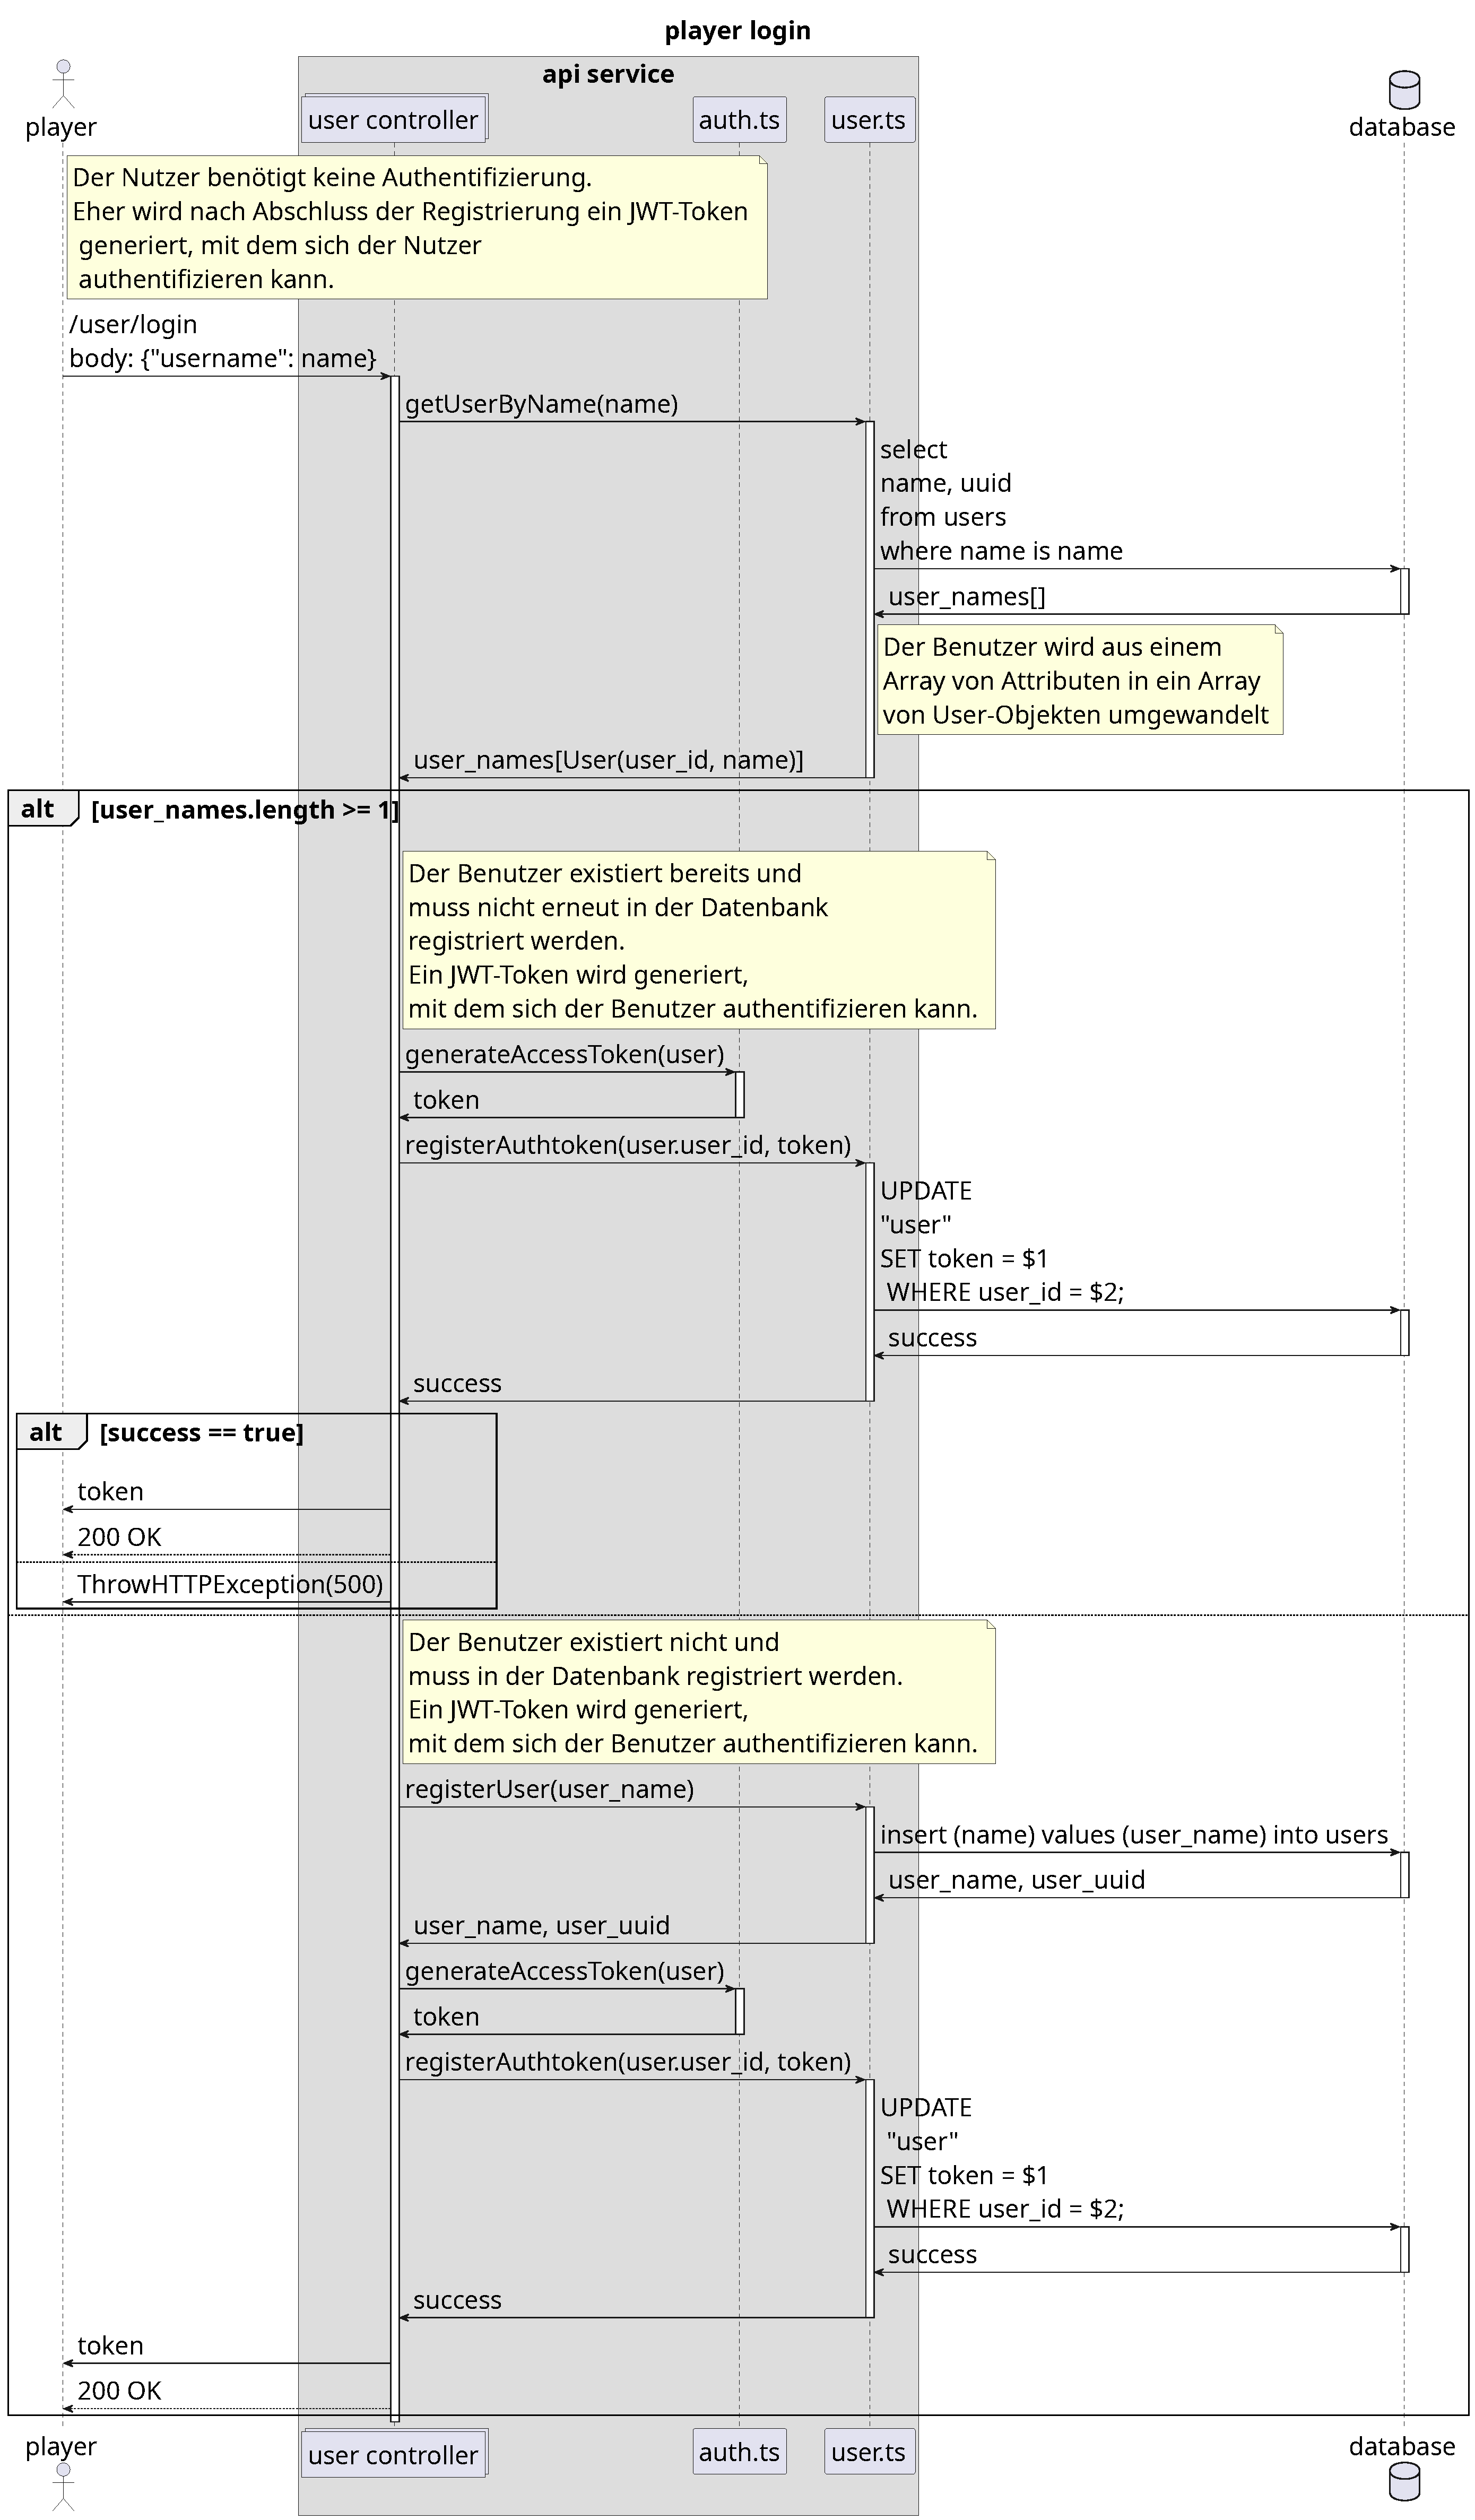
\includegraphics[width=\textwidth ]{resources/login.pdf}
	\caption{Zeigt den Ablauf einer Nutzerregestrierung.}
	\label{fig:ablaufdiagramm-login}
\end{figure}
\begin{figure}[H]
	\centering
	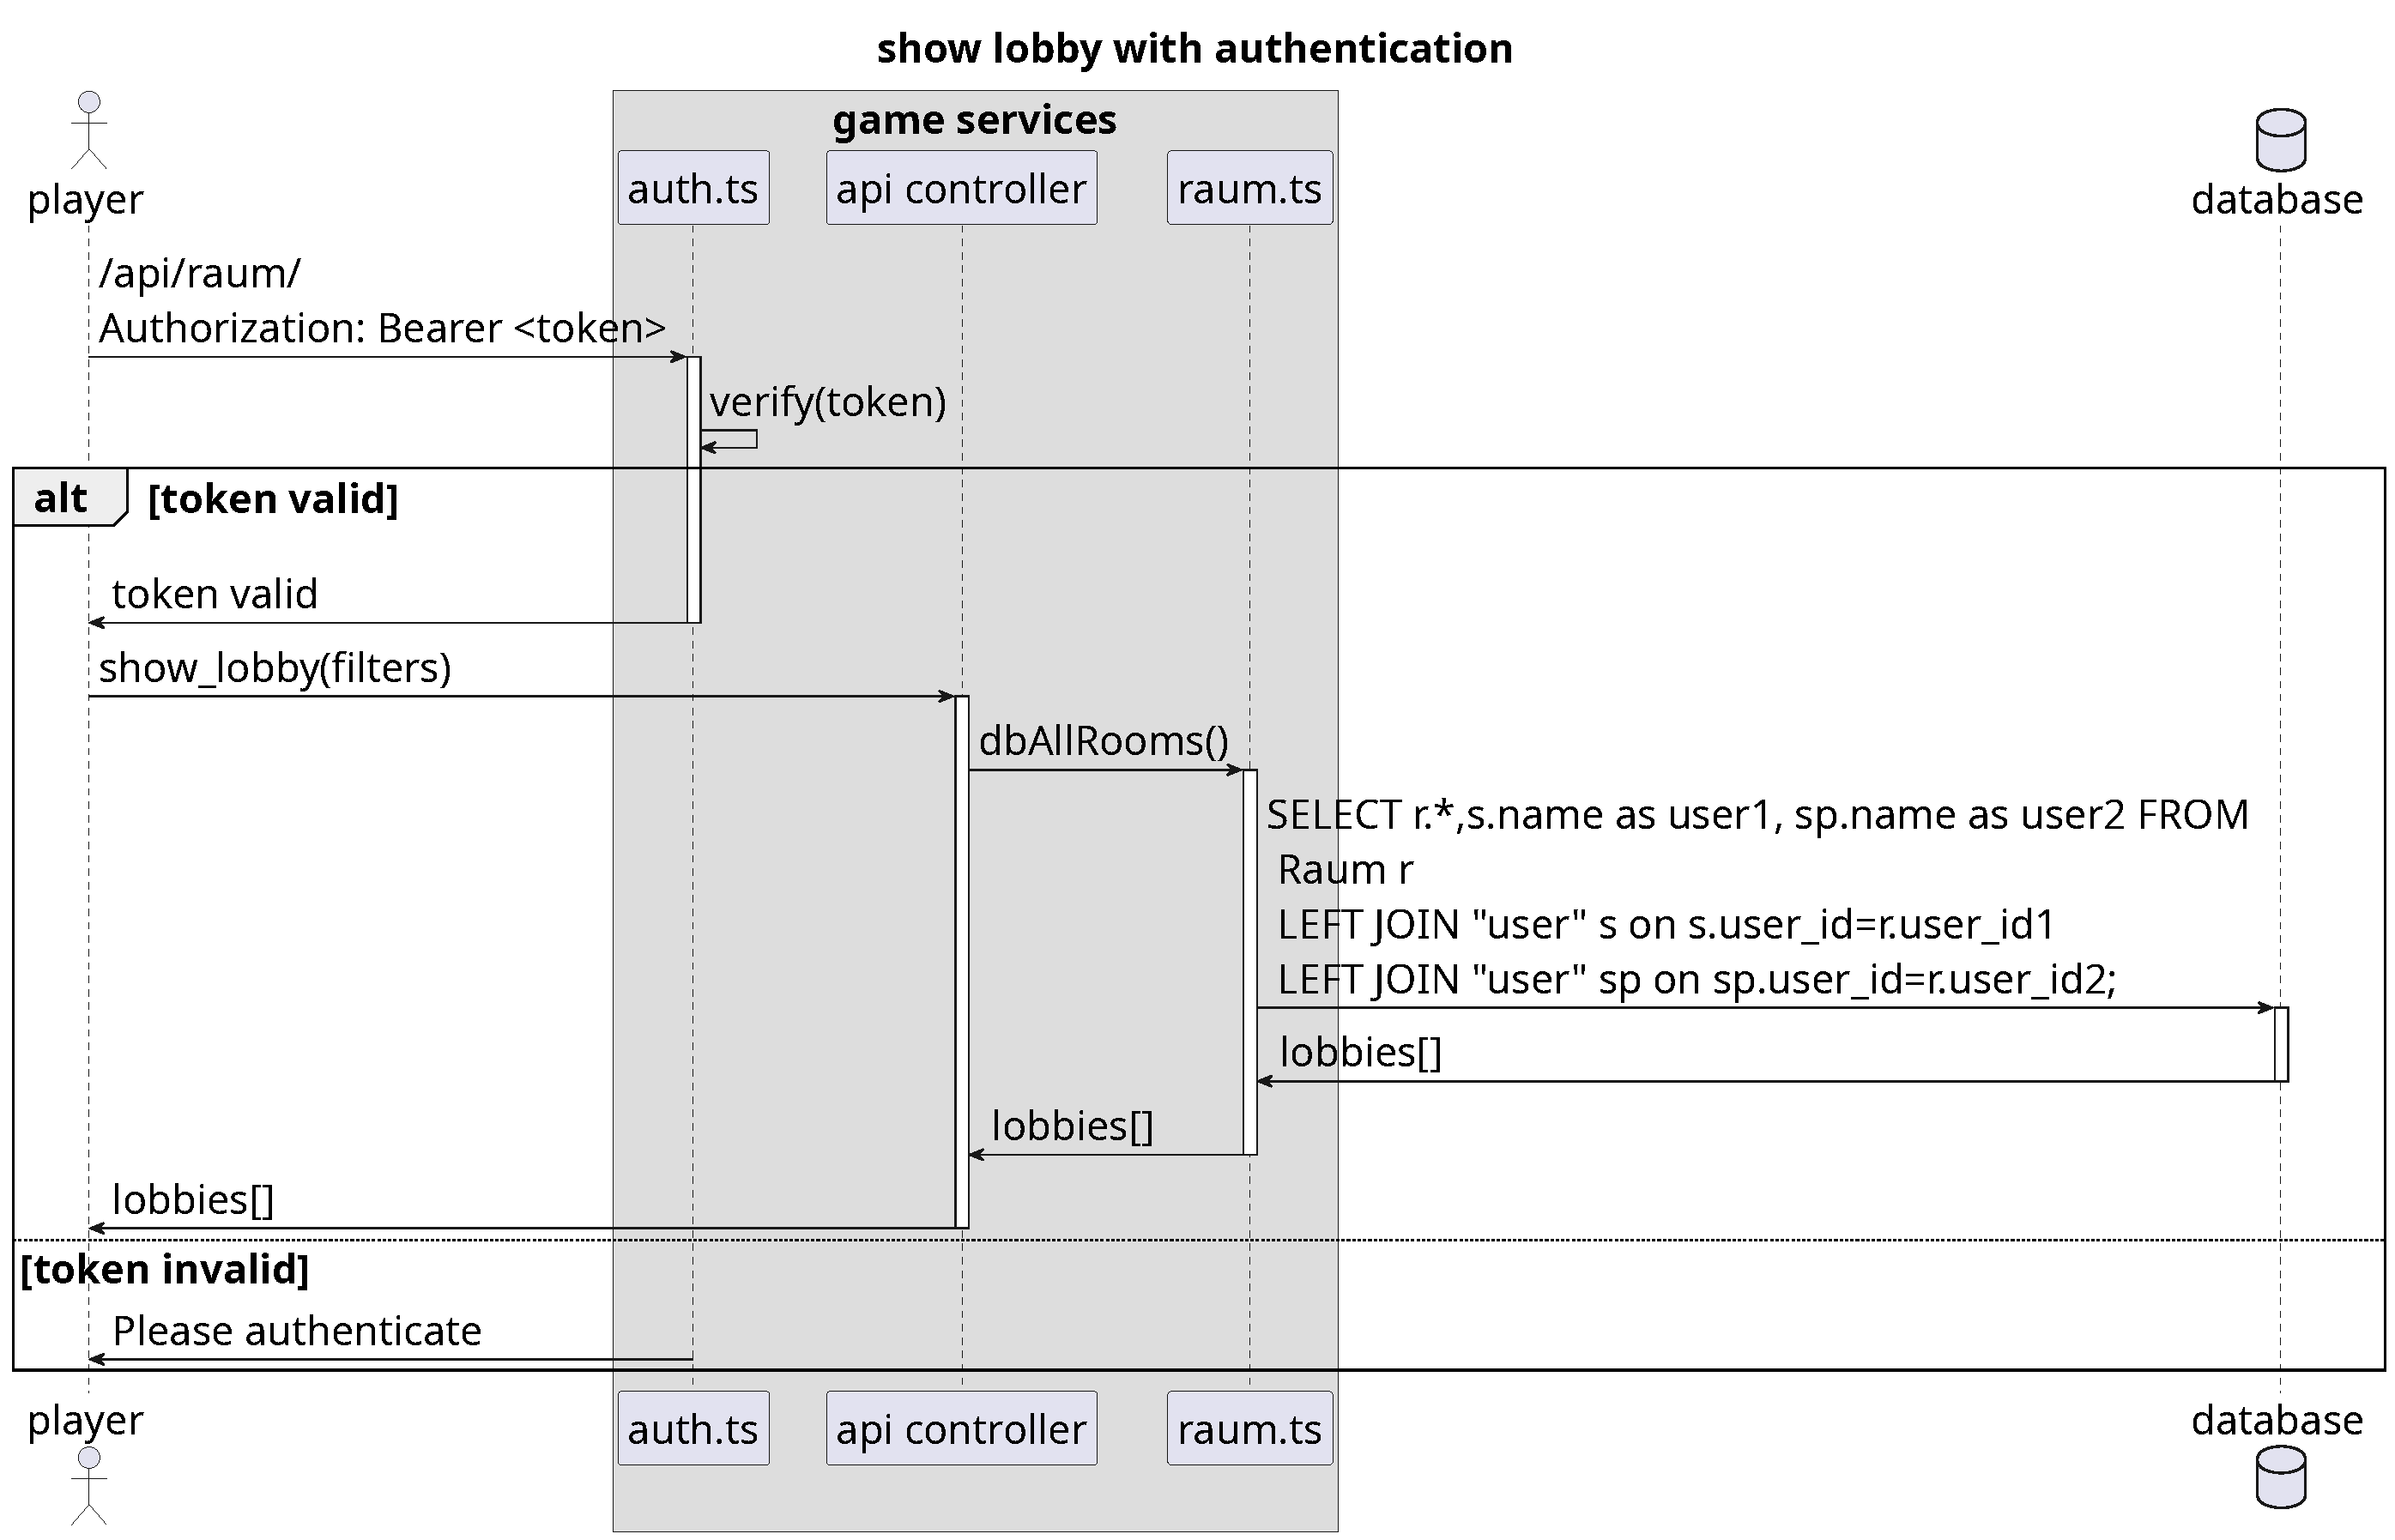
\includegraphics[width=\textwidth ]{resources/show_lobby.pdf}
	\caption{Zeigt den Ablauf der Abfrage aller Räume in der Datenbank. welche nach dem Login ausgeführt wird. Hier wir ein JWT-Token benötigt um die Anfrage zu autorisieren.}
	\label{fig:ablaufdiagramm-show_lobby}
\end{figure}
\begin{figure}[H]
	\centering
	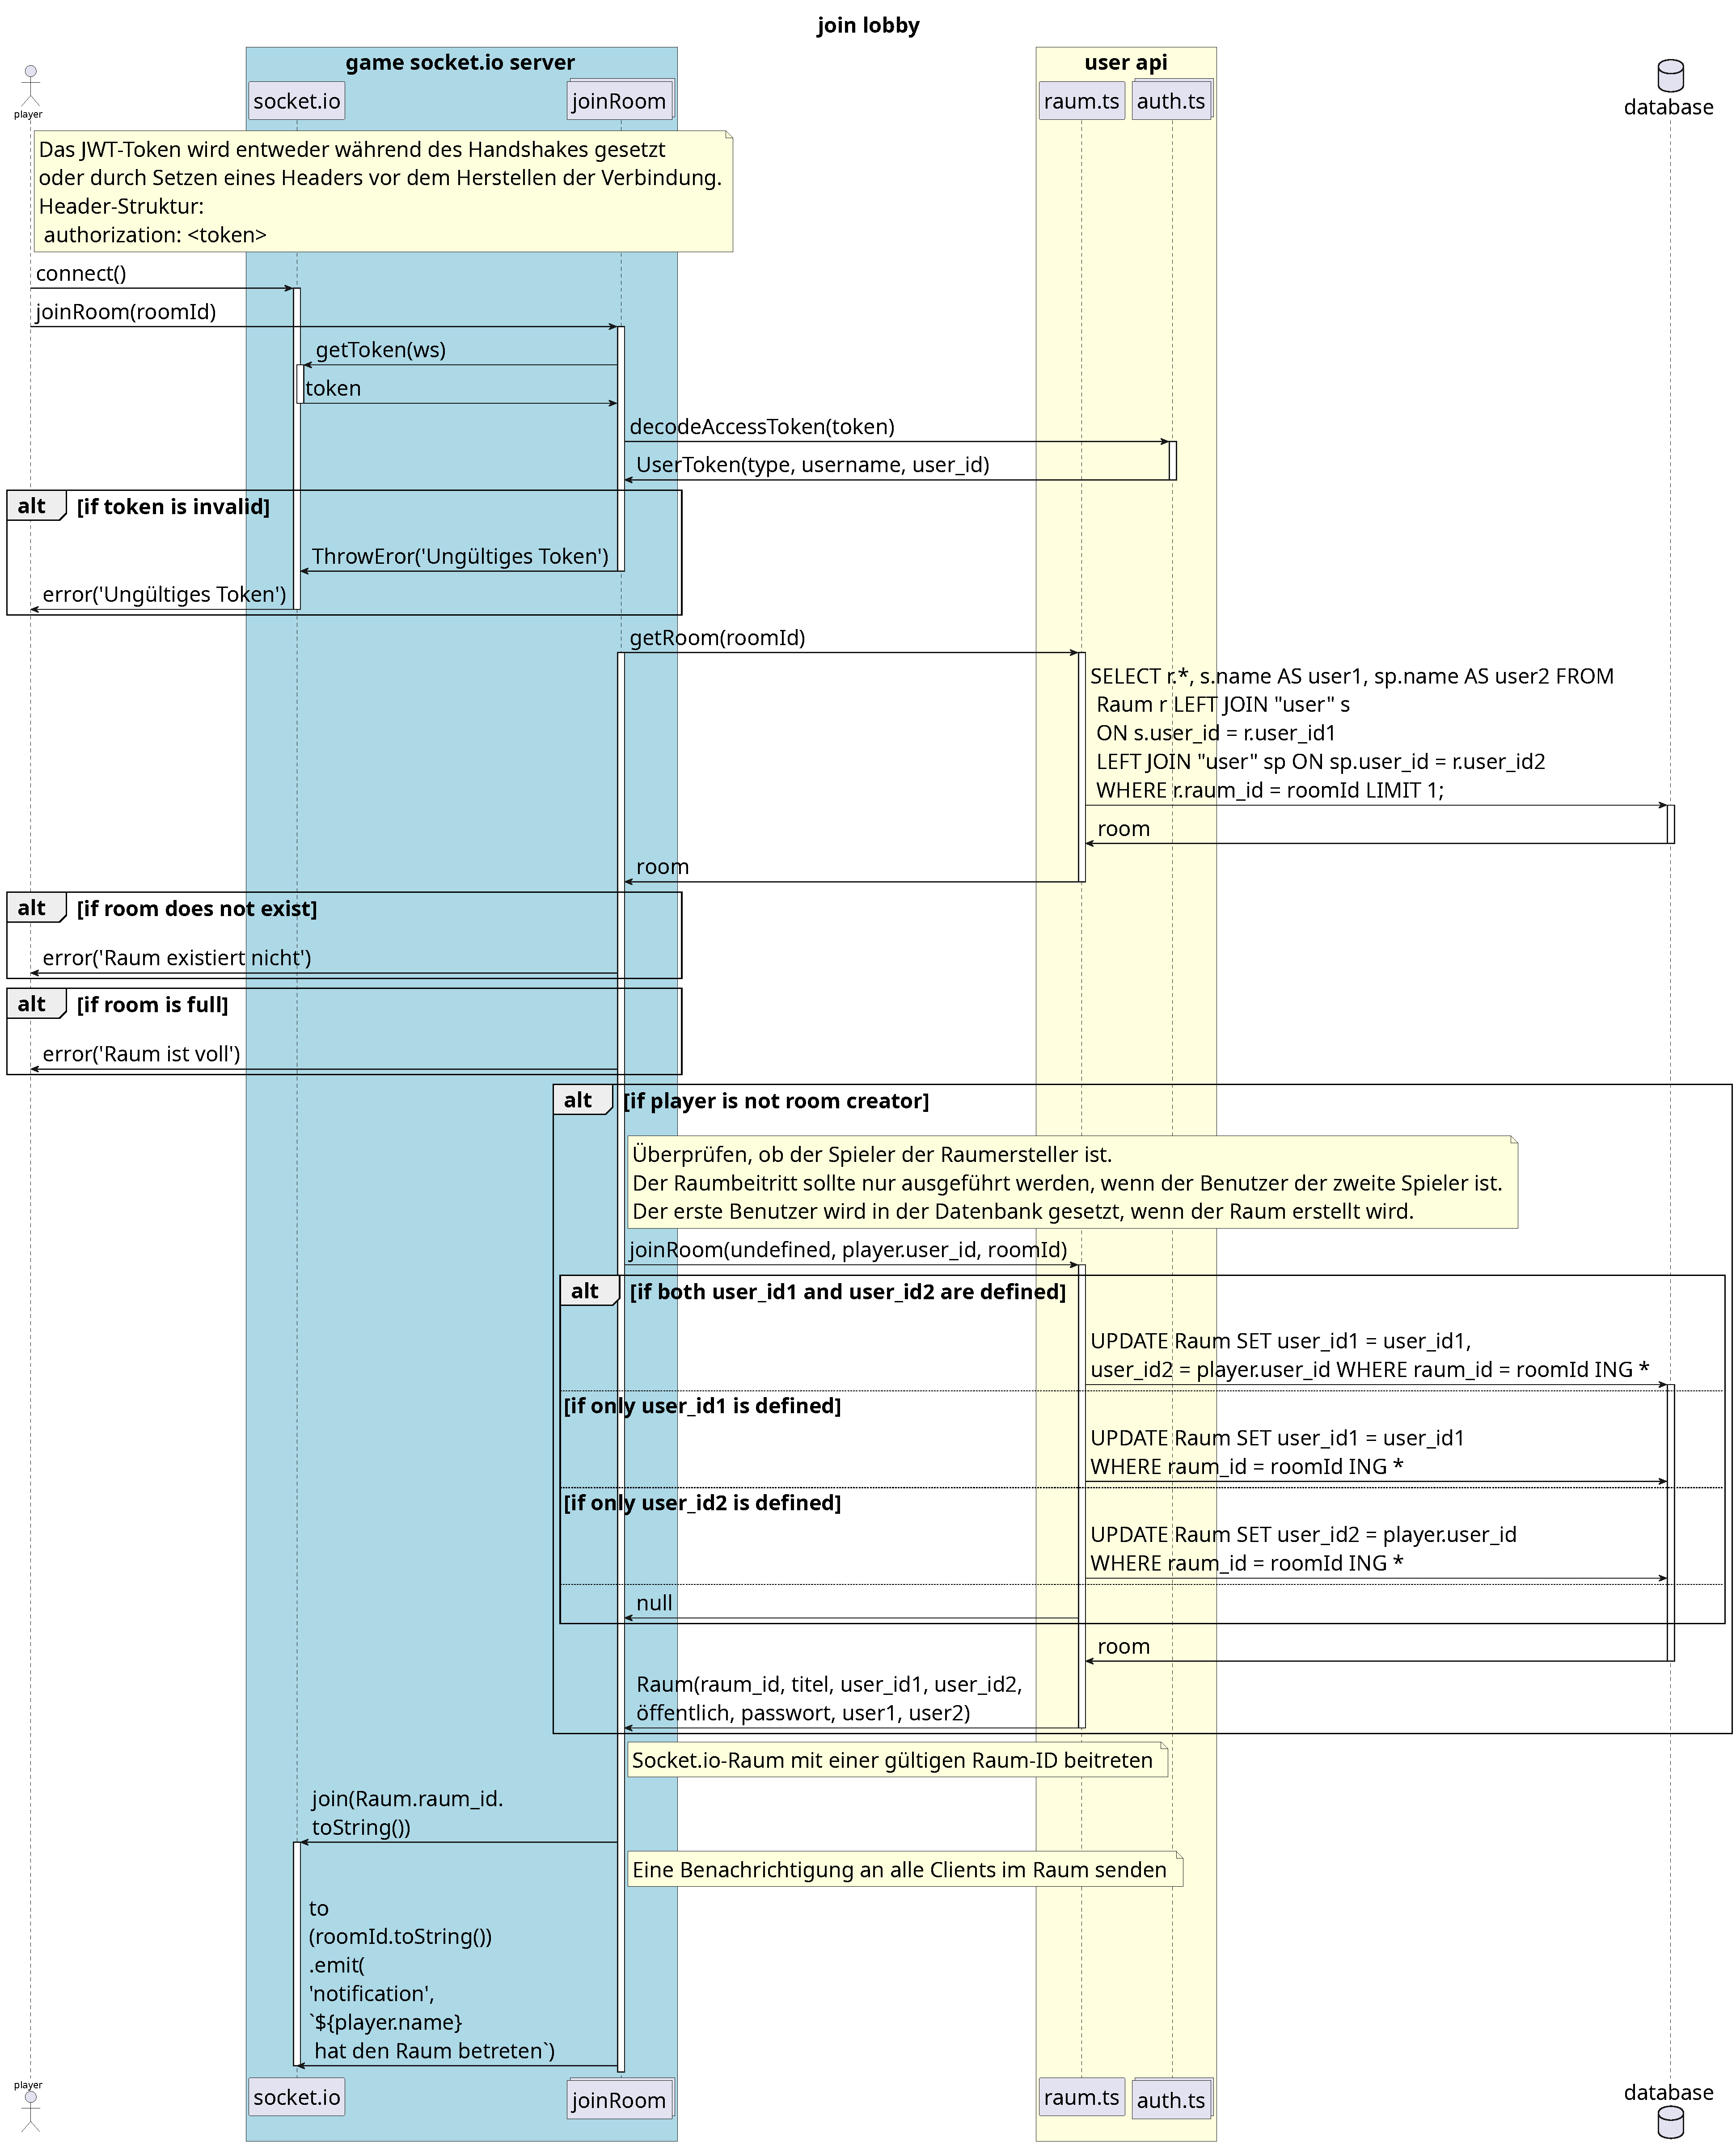
\includegraphics[width=\textwidth ]{resources/join_lobby.pdf}
	\caption{Der Nutzer tritt einem Raum bei. Hierbei wird ein JWT-Token benötigt um die Anfrage zu autorisieren. Der Nutzer verbindet sich mit dem Websocket und sendet eine joinRoom Anfrage. Der Server prüft ob der Nutzer die nötigen Berechtigungen hat um in den Raum beizutretten. Wenn der Nutzer alle Berechtigungen hat wird er in den Raum hinzugefügt und empfängt nun Nachrichten von anderen Nutzer.}
	\label{fig:ablaufdiagramm-join_lobby}
\end{figure}
\begin{figure}[H]
	\centering
	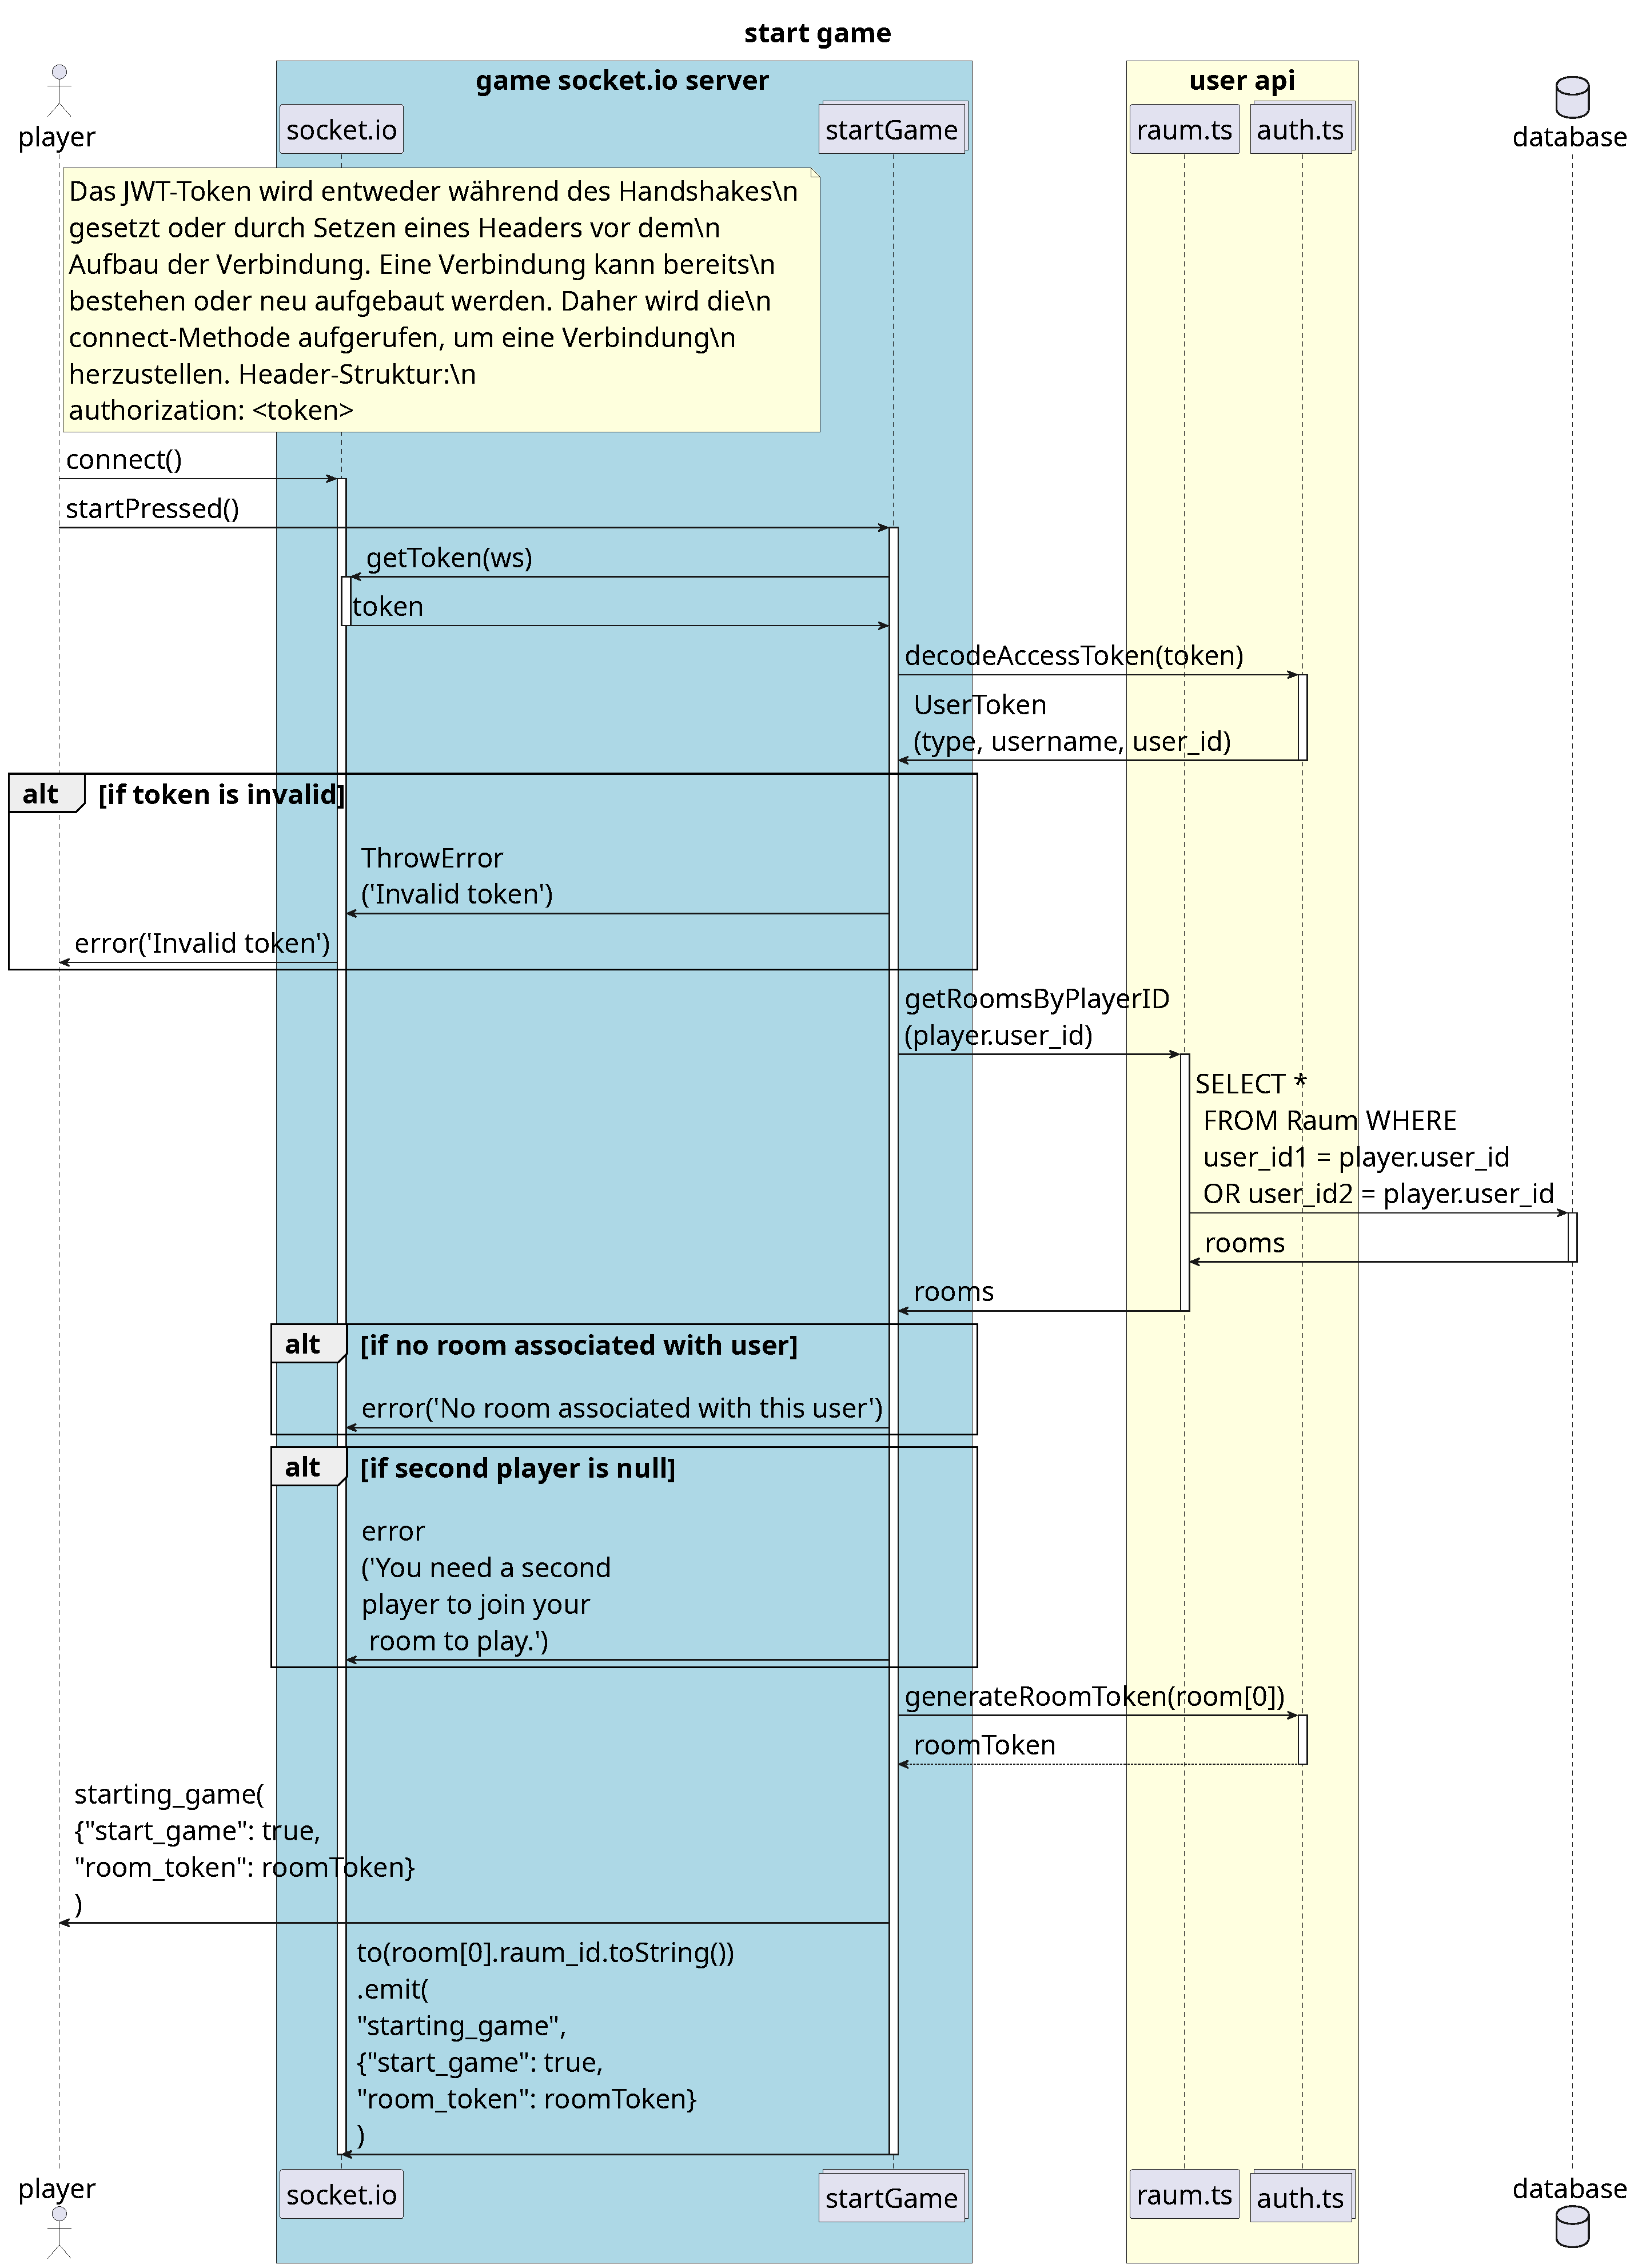
\includegraphics[width=\textwidth ]{resources/start_game.pdf}
	\caption{Drückt einer der Nutzer den Start-Button in der Benutzeroberfläche wird ein Event an den Server gesendet. Dieser Prüft ob der Nutzer innerhalb eines Raumes regestriert wurde. Wenn der Nutzer alle Berechtigungen erfüllt wird diesem ein Room Token übermittelt mit dem der Nutzer weitere Informationen authentifieren kann.}
	\label{fig:ablaufdiagramm-start_game}
\end{figure}

Wurde das Spiel gestartet wird bei jedem Client die Pong Instanz geladen. Die Kommunikation passiert über einen Socket-IO Websocket. Über den Socket senden die Clients dann verschiedene Events (ähnlich wie bei einem Publisher/Subscriber Prinzip \cite{tanenbaum2007distributed}) welche dann auf der anderen Seite interpretiert werden. Die Clients senden nun die Positionen ihrer Paddles an den Server welcher diese an die Clients weitergibt. Prallt ein Ball an einem Paddle ab meldet der Client an dem der Ball abgeprallt ist dass dieser abgeprallt ist. Genauso passiert das, wenn ein Tor geschossen wird (vgl. Abbildung \ref{fig:ablaufdiagramm-spiel}). 
\begin{figure}[H]
	\centering
	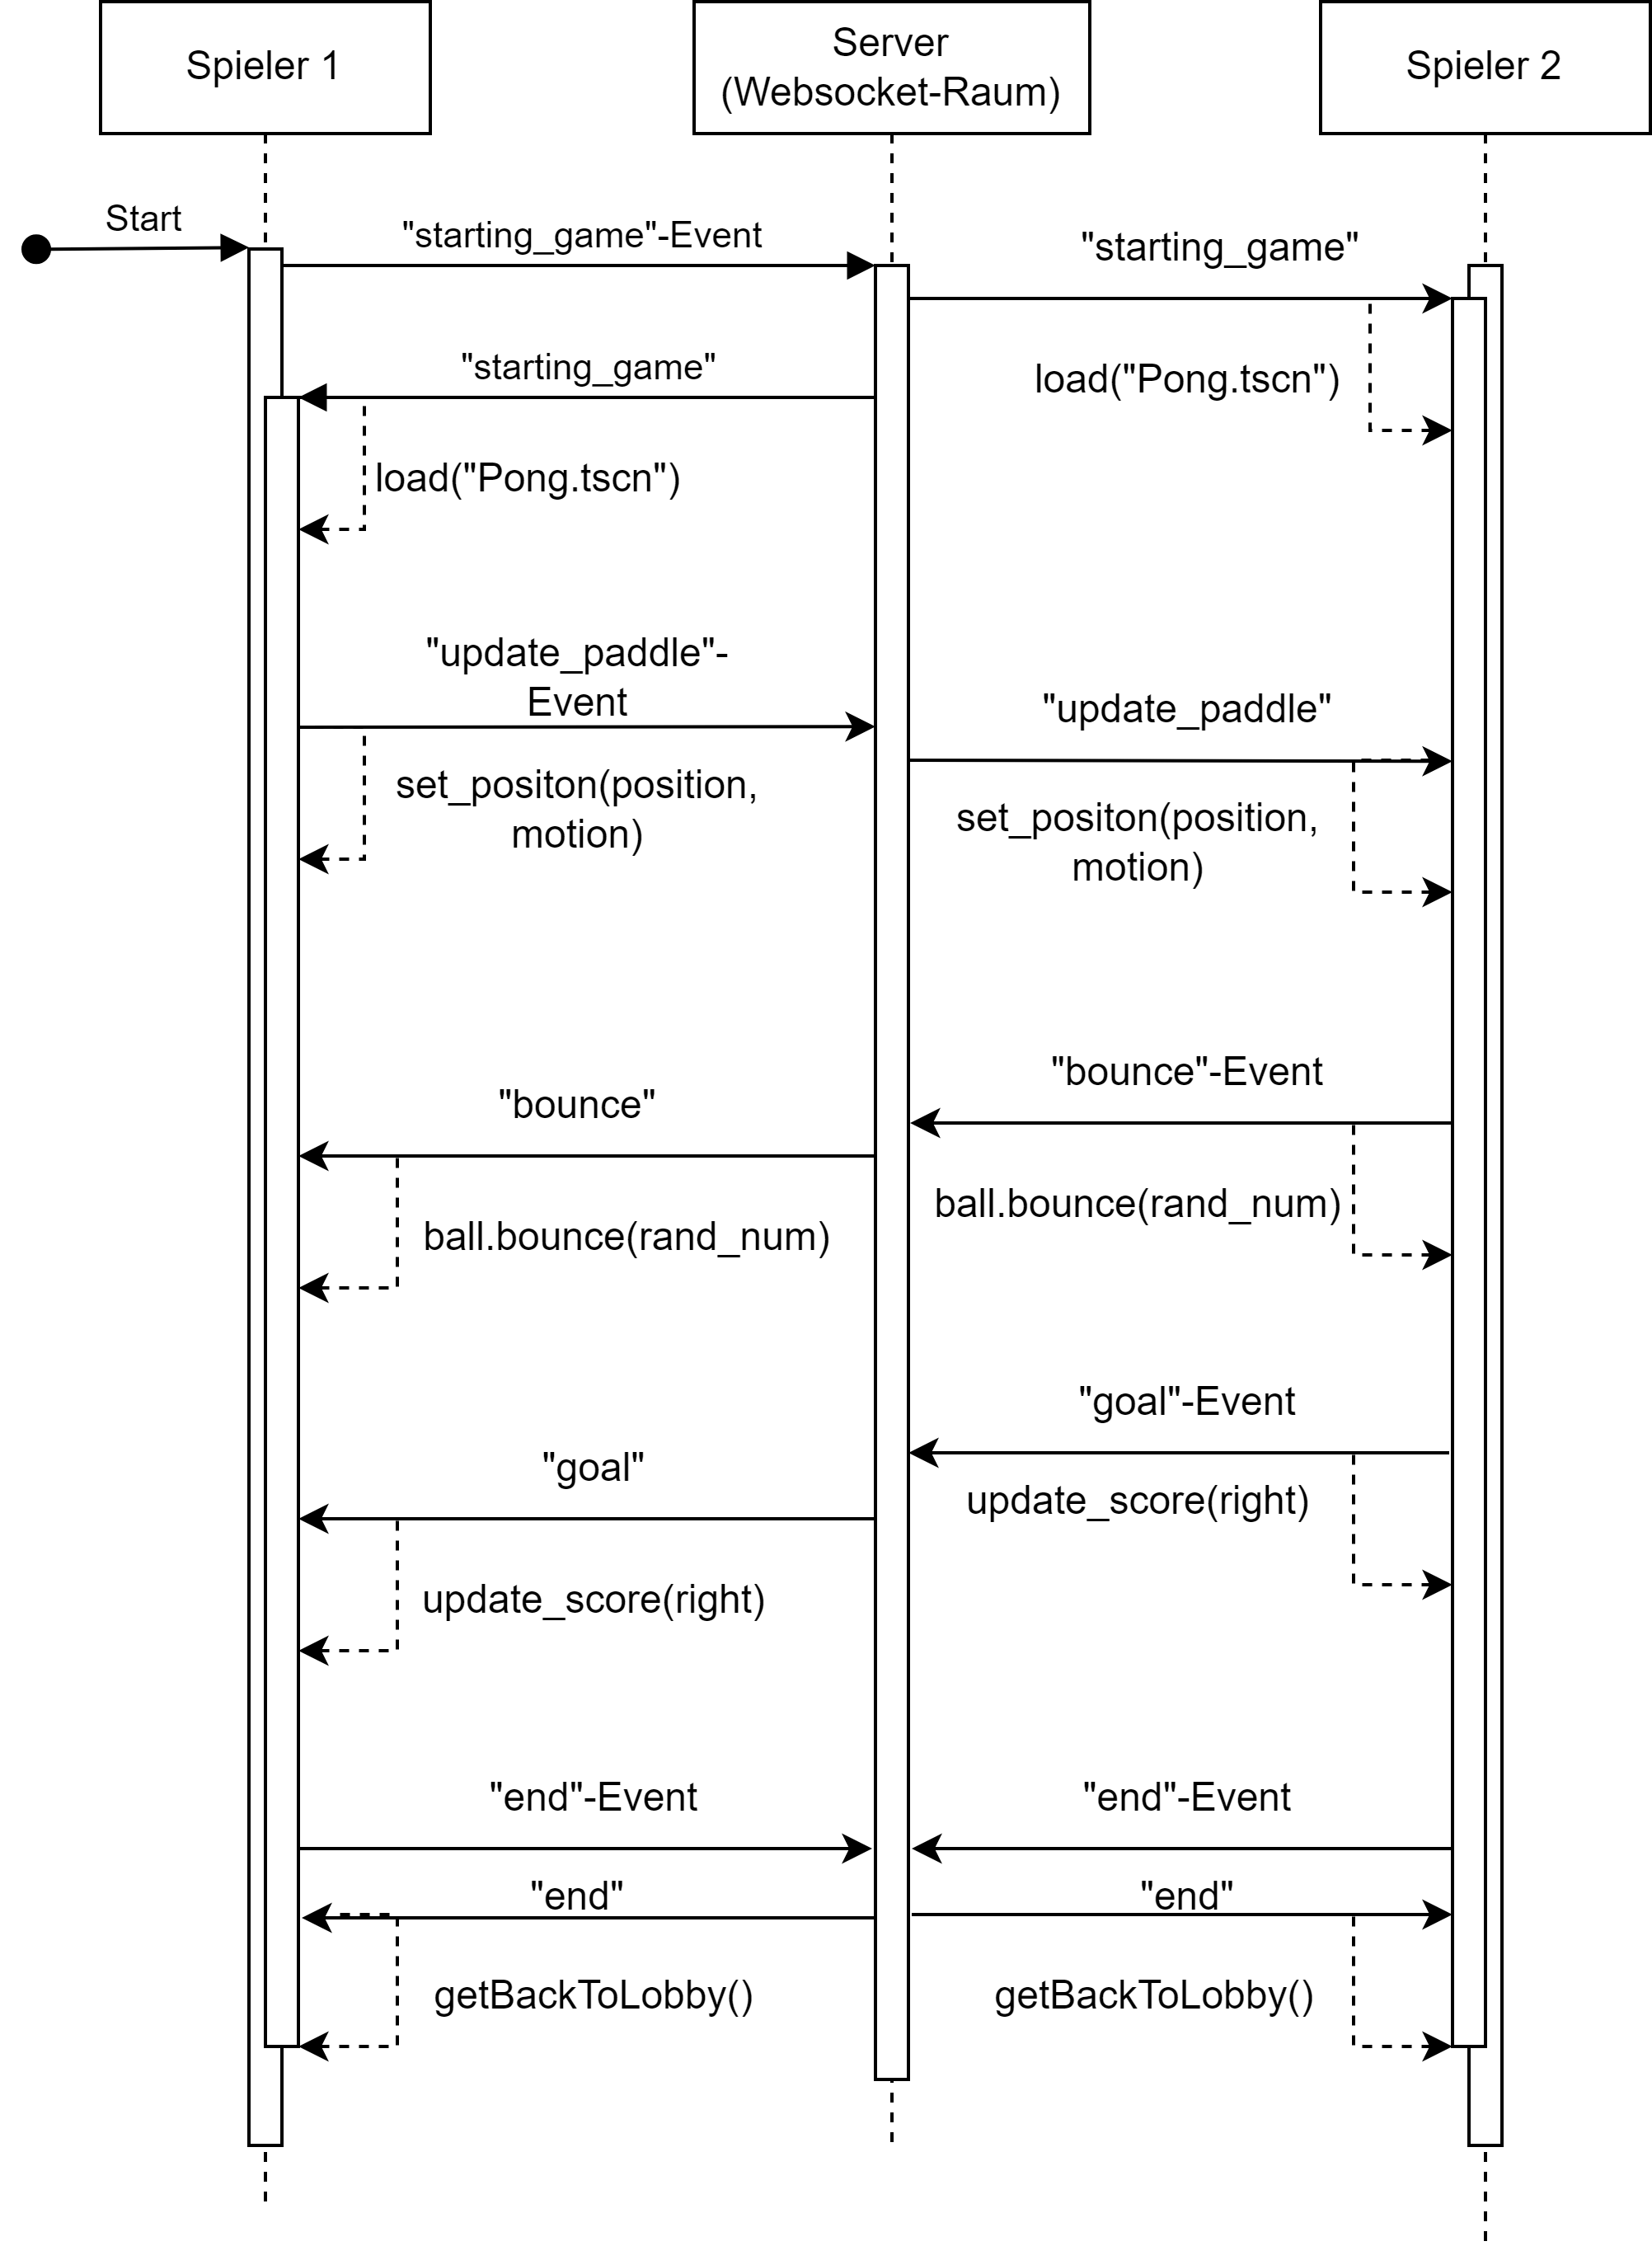
\includegraphics[width=\textwidth -120pt ]{resources/Event-Based-Spielablauf.png}
	\caption{Eventbasierter Ablauf des Spiels über einen Socket-IO Websocket. Es handelt sich um eine Vereinfachte Ansicht. Beide Seiten können die jeweiligen Events an den Server senden.}
	\label{fig:ablaufdiagramm-spiel}
\end{figure}
Einer der Schwierigkeiten waren stockende Bewegungen vom Ball während des Spielablauf. Um dem Problem entgegenzuwirken, rendert jeder Client den Ball für sich selbst und nur die Änderungen, z.B. beim Aufprall werden übertragen. 
Außerdem musste sichergestellt werden, dass jeder Raum über einen sepearaten Channel kommuniziert. Hierfür eignete sich das Raum-Management Feature von Socket-IO , da die Verbindung \& Synchronisation schon übernommen wurde und man einfach die Raum ID's aus der Datenbank sehr einfach einbinden konnte. So konnte ein höherer Programmieraufwand und damit Potenzielle Fehler vermieden werden \cite{SocketIORooms}. 

\subsection{Mögliche Alternativen}
Anstelle einer zentralisierten Architektur wäre ein dezentralisierter Ansatz möglich. Es könnte ein Peer-To-Peer System Implementiert werden. Anstelle von einem zentralen System ist jeder Client miteinander direkt verbunden \cite{gordon2001distributed}. Im folgenden werden die Vor- und Nachteile eines Peer-To-Peer Systems erläutert:

\textbf{Vorteile}
\begin{itemize}
\item Geringere Latenz wenn die zwei Spieler eine direkte Verbindung zueinander herstellen
\item Ein Load Balancer wird nicht benötigt da jeder Client seine eigenen Ressourcen mitbringt und die Spiellogik dann von Peer to Peer abläuft
\end{itemize}

\textbf{Nachteile}
\begin{itemize}
\item Synchronisation ist bei einem P2P-Netzwerk komplexer herzustellen, anstatt mit einem zentralisiertem Server
\item Firewalls \glqq erschweren\grqq{} den Datenaustausch wenn ein Client keine Verbindung zulässt \cite{gordon2001distributed}
\end{itemize}

\section{Reflexion}

\subsection{Rückblick \& Hearusforderungen}
\begin{itemize}
    \item \textbf{Änderungen nach dem Projekt}: Was würde man im Nachhinein anders machen, um das System zu verbessern?
      \item \textbf{Größte Herausforderungen}: Rückblick auf die bedeutendsten Schwierigkeiten und wie sie gelöst wurden.
\end{itemize}
Rückblickend gesehen wäre es besser gewsesen die gesamte Logik der Raumliste mit Websockets aufzubauen. Anstatt die Räume mit einer REST-API abzufragen, könnten Aktualisierungen der Räume in Echtzeit übertragen werden. So müsste der Benutzer nicht Manuell die Räume abfragen und potenzielle Race-Conditions, wie beim Raumbeitritt könnten vermieden werden. Außerdem müssten damit nicht die gesamten Räume vom Server gefetcht werden sondern es könnte zu Beginn einmal alles gefetcht werden und nur noch Änderungen müssten übertragen werden.   
Eine große Herausforderung war außerdem die Verwendung der Programmiersprache Typescript. Da alle Teilnehmer des Projektes nahezu keine Erfahrung mit Typescript hatten, ist viel Zeit drauf gegangen um Bugs zu fixen welche aufgrund vom Datentypen handling der Programmiersprache entstanden sind. In Zukunft wird für das Backend eine andere Sprache verwendet.

Für die Verwaltung von Daten wäre eine objektorientierte Datenbank wie z.B. MongoDB besser geeignet gewesen, da 
Trash Pong die Komplextät für eine relationale Datenbank nicht mitbringt. 
\newpage
 \printbibliography[title={Quellen}]
\end{document}
